% Compile: lualatex paper_en.tex
\documentclass[10pt,twocolumn]{article}
\usepackage{fontspec}
\usepackage[a4paper,margin=18mm]{geometry}
\usepackage{graphicx}
\usepackage{amsmath}
\usepackage{amssymb}
\usepackage{booktabs}
\usepackage{enumitem}
\usepackage{microtype}
\usepackage[hidelinks]{hyperref}
\usepackage{titlesec}
\titleformat*{\section}{\large\bfseries}
\titleformat*{\subsection}{\normalsize\bfseries}

\setlength{\columnsep}{6mm}
\setlength{\parskip}{2pt}

\begin{document}

\twocolumn[{%
  \begin{center}
    {\LARGE\bfseries Character LoRA Fine-tuning of a 33B Omni-modal Video Model}\\
    \vspace{0.6em}
    {\large ---System RAM, Not VRAM, Was the Binding Constraint---}\\
    \vspace{1.2em}
    {\large Masato Suzuki (Masafy)}\\
    \vspace{0.4em}
    {15 August 2026}
  \end{center}
  \vspace{1.0em}
  {\centering\textbf{Abstract}\par}
  \vspace{0.4em}
  \begingroup\small
  \noindent This report extends the author's earlier work---character LoRA fine-tuning of Stable Diffusion~1.5 (about 1B parameters)~\cite{suzuki2026sd15lora} and of Krea~2 (about 12B)~\cite{suzuki2026krea2lora}---into video generation. The target is \textbf{MiniMax~H3}, an omni-modal model that generates video and audio jointly, with a diffusion transformer of roughly 33B parameters paired with a 32B Qwen3-VL text encoder. The subject is the same original character (a red panda, ``Masafy'') used in both earlier studies. Those two studies each concluded that a single consumer GPU with 12\,GB of VRAM suffices; \textbf{here the same GPU did not suffice}. Tracing the failure by measurement showed that the binding constraint is not VRAM but \textbf{system RAM}. Peak VRAM during training measured 3{,}959\,MiB---2.8\% of the card actually used---while loading the 41.2\,GB model set failed three times by OOM on hosts with 50\,GB of system RAM and completed on a host with 188\,GB. We further show that (a) the trained adapter transfers across quantization formats (trained on pruned INT8, applied to GGUF~Q3\_K\_M, all 208 modules matching) and runs inference within 9.3\,GB of VRAM; (b) with a reference-image conditioning scheme, the LoRA contributes \emph{style} rather than structural stability; and (c) adapter strength trades style fidelity against structural accuracy, with a cross-validated optimum at 500 steps and strength 0.8. Total compute cost was about five US dollars.

  \par\medskip
  \noindent\textbf{Keywords:}\ video generation, omni-modal models, diffusion transformer, low-rank adaptation, LoRA, system memory, quantization, consumer GPU, reproducibility
  \endgroup
  \vspace{2.0em}
}]

\section{Introduction}

In two earlier studies the author fine-tuned an original character---``Masafy'', a red panda---into Stable Diffusion~1.5~\cite{suzuki2026sd15lora} and then Krea~2~\cite{suzuki2026krea2lora} using low-rank adaptation (LoRA)~\cite{hu2022lora}, each time on a single consumer GPU with 12\,GB of VRAM. The second study combined FP8 quantization with block swapping to bring a 12B model---roughly 24\,GB of weights at half precision---inside a 12\,GB card.

Together these results supported a general claim: \emph{with the right techniques, personal fine-tuning of a current generative model fits on one consumer GPU.} This study asks whether the claim survives the move to \textbf{video generation}.

MiniMax~H3 generates video and audio jointly. Its diffusion transformer holds roughly 33B parameters and it pairs with the 32B variant of the Qwen3-VL text encoder. It offers Reference-to-Video-Audio (R2V) conditioning, which pins a character from a reference image.

The research questions are:

\begin{itemize}[leftmargin=2.2em,topsep=2pt,itemsep=1pt]
  \item[\textbf{Q1.}] On the same 12\,GB GPU used before, can a 33B-class video model be LoRA-trained? If not, what is the real constraint?
  \item[\textbf{Q2.}] Does the trained adapter transfer to an inference stack that uses a different quantization? What does inference cost?
  \item[\textbf{Q3.}] When a reference image already pins the character, what does the LoRA add? Where are the best strength and training length?
\end{itemize}

\textbf{The main contribution is a negative answer to Q1 together with the identification of its cause}---the author marking the boundary of a claim his own earlier work established.

\section{Setup}

\subsection{Model composition}

Table~\ref{tab:model} lists the components. The text encoder alone is 32B; with the transformer, loading amounts to a 65B-class set of weights. That fact is the direct cause of the constraint reported below.

\begin{table}[t]
\centering\small
\caption{Model composition}
\label{tab:model}
\begin{tabular}{lr}
\toprule
Component & Size \\
\midrule
Transformer (pruned INT8 ConvRot) & 20.0\,GB \\
Text encoder (Qwen3-VL 32B) & 15.7\,GB \\
VAE (video fp16 / audio fp32) & 5.5\,GB \\
\midrule
Total & 41.2\,GB \\
\bottomrule
\end{tabular}
\end{table}

\subsection{Training configuration}

Training used ai-toolkit~\cite{aitoolkit2026} pinned at commit \texttt{f4e9130}. The LoRA is rank~16 / alpha~16 over \texttt{attn.qkv\_proj}, \texttt{attn.out\_proj}, \texttt{mlp.fc1} and \texttt{mlp.fc2}, reaching \textbf{208 modules} (416 tensors) across 50 blocks plus the token refiner.

The dataset is 12 training images, 2 validation and 2 excluded, each 1000$\times$1000, drawn by the author. Frame count is 1---stills treated as single-frame video---with batch size 1, gradient checkpointing on, bf16, at resolutions 512 and 768.

Every caption opens with \texttt{masafy\_character,} followed by the fixed appearance (aviator goggles, patterned scarf) and then a per-image description of pose, expression and background. Caption dropout is 0.05.

\begin{figure*}[t]
\centering
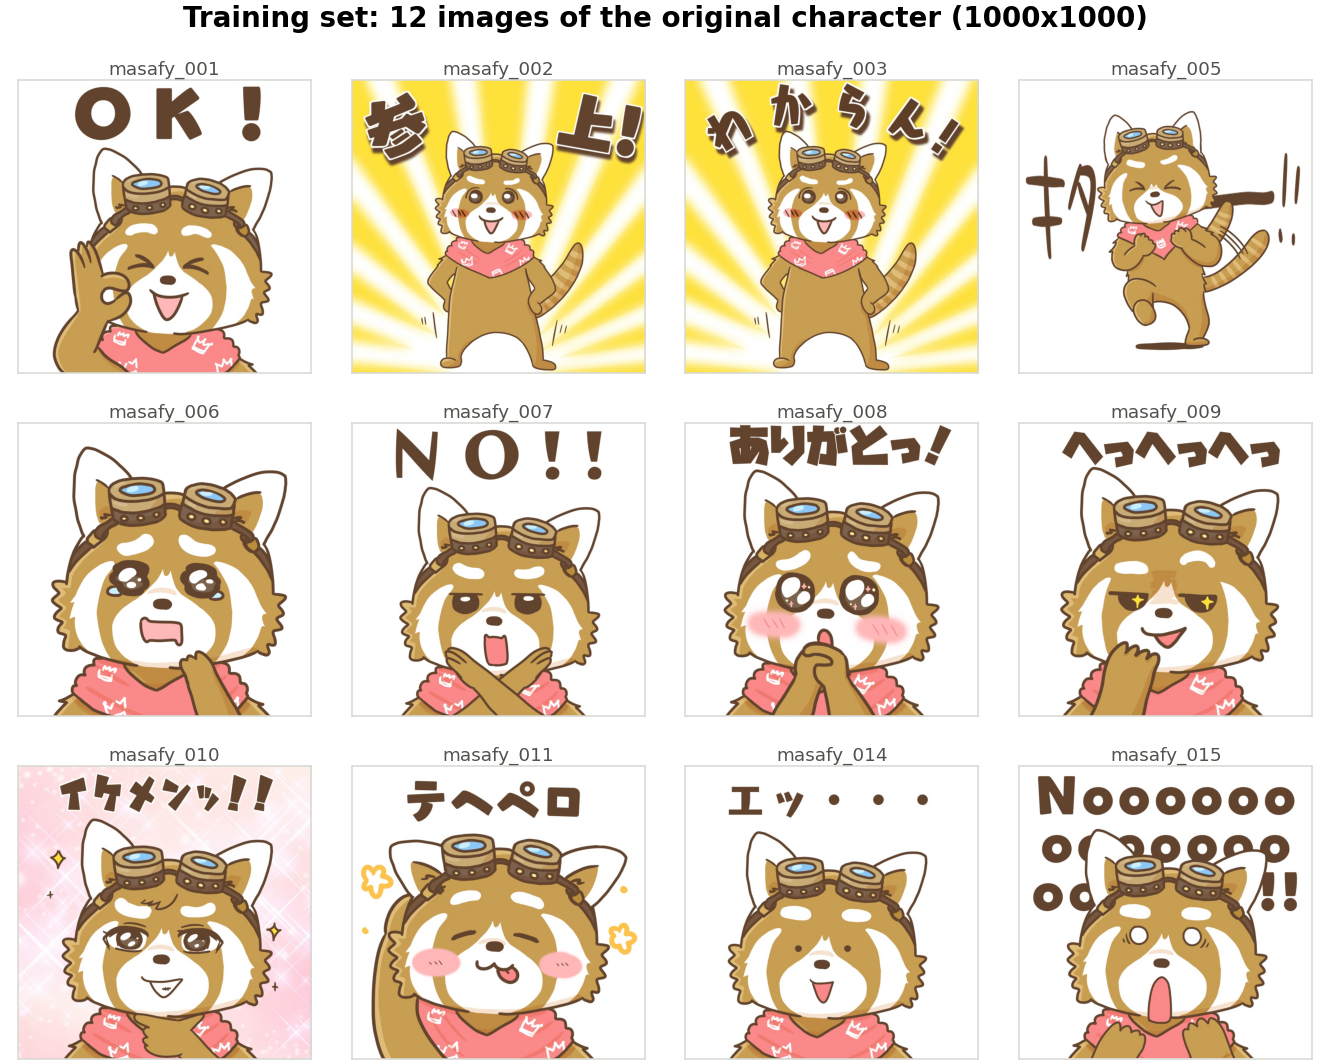
\includegraphics[width=\linewidth]{figures/fig_dataset.png}
\caption{The training set: 12 images of the character drawn by the author. Most carry the die-cut border of their original sticker use.}
\label{fig:dataset}
\end{figure*}

\subsection{Environments}

Four environments were tried (Table~\ref{tab:env}). Recording \emph{both} VRAM and system RAM is the methodological point of this study.

\begin{table*}[t]
\centering\small
\caption{Environments and outcomes. VRAM does not predict success; system RAM does.}
\label{tab:env}
\begin{tabular}{llrrrl}
\toprule
Environment & GPU & VRAM & System RAM & Price & Outcome \\
\midrule
Local & RTX 3060 & 12\,GB & 30\,GB & electricity & fail (0 steps in 2h25m) \\
Cloud A & A40 & 48\,GB & 50\,GB & \$0.44/h & fail (OOM, \texttt{low\_vram} on) \\
Cloud A$'$ & A40 & 48\,GB & 50\,GB & \$0.44/h & fail (OOM, \texttt{low\_vram} off) \\
Cloud B & H200 SXM & 141\,GB & 233\,GB & \$4.59/h & success (pilot) \\
Cloud C & RTX 6000 Ada & 48\,GB & 188\,GB & \$0.84/h & success (full run) \\
\bottomrule
\end{tabular}
\end{table*}

\section{Q1: Identifying the constraint}

\subsection{Failure on the local GPU}

On the RTX 3060 (12\,GB VRAM, 30\,GB RAM) used in both earlier studies, a pilot run \textbf{completed zero steps in two hours and twenty-five minutes}. GPU utilization read 0.0\% at every sample; the run halted just after \texttt{Quantizing transformer} and produced nothing.

Utilization pinned at zero means the GPU was not waiting on compute---the run never reached compute. The \texttt{low\_vram} path offloads weights to the host, but 41.2\,GB of weights against 30\,GB of RAM pushes the remainder into swap.

The first lesson follows: \textbf{the existence of a \texttt{low\_vram} option does not imply the run will work.} Check that system RAM can hold the whole model before checking VRAM at all.

\subsection{Reproducing and isolating the failure}

On 48\,GB VRAM / 50\,GB RAM the run died at the same point both times, killed by signal (exit 137):

\begin{quote}\small\ttfamily
Loading Qwen3-VL text encoder\\
 - attached 351 pre-quantized layers\\
Text encoder is already quantized\\
Killed
\end{quote}

After the 20.0\,GB transformer, adding the 15.7\,GB text encoder reaches 36\,GB; runtime overhead carries it past the 50\,GB ceiling.

Crucially, the second attempt with \texttt{low\_vram} \emph{disabled} failed \textbf{at the same point}. Weights are staged in host RAM before transfer to the device, so the failure is independent of free VRAM---which indeed measured 0--3\,MiB at that moment.

Hosts with 188\,GB and 233\,GB both completed. The requirement therefore lies \textbf{above 50\,GB and at or below 188\,GB}.

Figure~\ref{fig:constraint} plots VRAM and system RAM against outcome. Two 48\,GB hosts sit on opposite sides of the outcome column, so VRAM carries no signal; system RAM separates cleanly between 50 and 188.

\begin{figure*}[t]
\centering
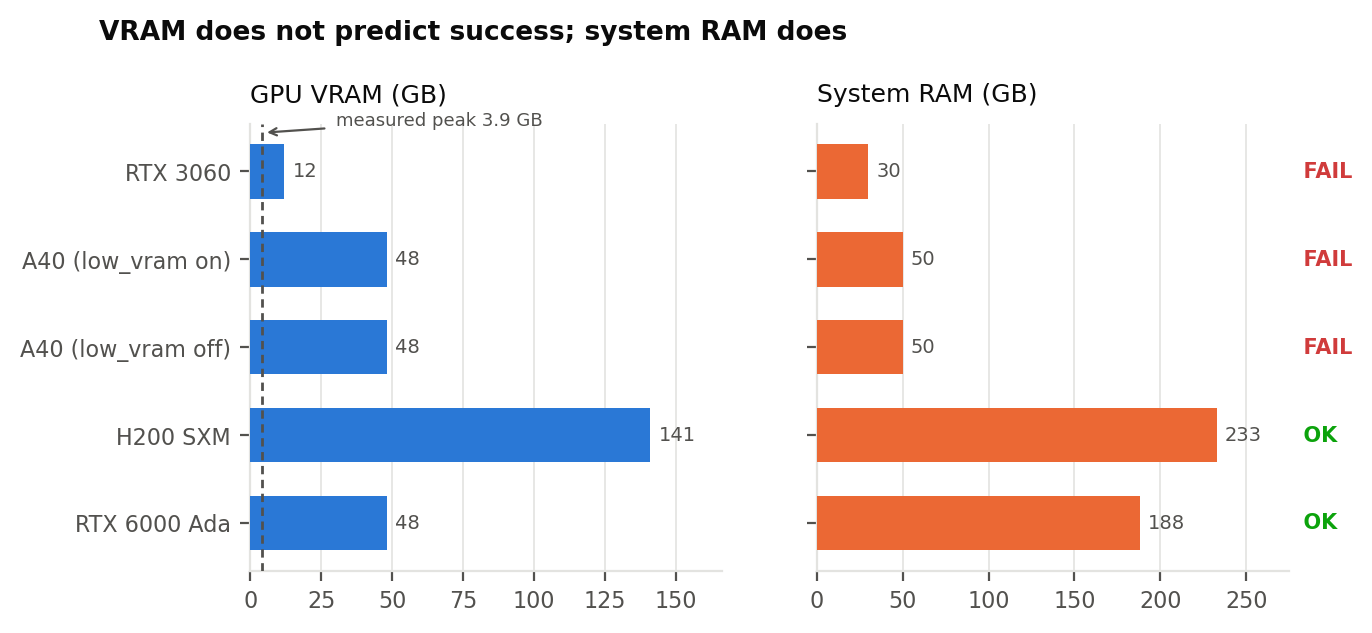
\includegraphics[width=\linewidth]{figures/fig_constraint.png}
\caption{VRAM does not predict success; system RAM does. The dashed line marks measured peak VRAM during training (3.9\,GB).}
\label{fig:constraint}
\end{figure*}

\subsection{RAM allocation does not track price}

Surveying commercial offerings shows that system RAM correlates with neither price nor VRAM (Table~\ref{tab:ram}).

\begin{table}[t]
\centering\small
\caption{Advertised host allocations}
\label{tab:ram}
\begin{tabular}{lrrr}
\toprule
GPU & VRAM & System RAM & Price \\
\midrule
RTX 3090 & 24\,GB & 125\,GB & \$0.50/h \\
RTX 4090 & 24\,GB & \textbf{41\,GB} & \$0.69/h \\
RTX 6000 Ada & 48\,GB & 167\,GB & \$0.84/h \\
A40 & 48\,GB & \textbf{50\,GB} & \$0.44/h \\
H100 NVL & 94\,GB & \textbf{94\,GB} & \$3.19/h \\
\bottomrule
\end{tabular}
\end{table}

The RTX 4090 costs more than the 3090 and ships a third of its RAM. The original plan called for a 4090; none was in stock. \emph{Had one been available, the run would have failed earlier than it did on the A40.}

Allocations also vary within a single GPU model depending on the hosting tier. Third-party-hosted RTX 3090 instances measured 30\,GB and 41\,GB of RAM against an advertised 125\,GB (two independent draws).

\subsection{The successful run}

On the RTX 6000 Ada (188\,GB RAM, \$0.84/h), 800 steps took 9.04\,s per step, stable to the last step, for a wall clock of 2h00m15s at \$1.89. Figure~\ref{fig:loss} shows the loss trace.

\begin{figure}[t]
\centering
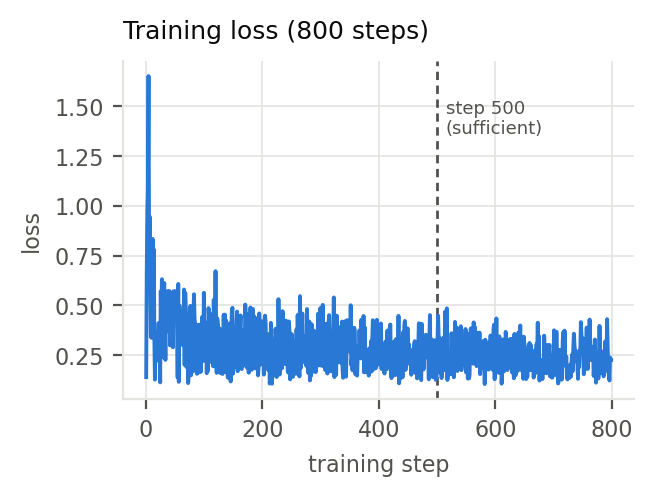
\includegraphics[width=\linewidth]{figures/fig_loss.png}
\caption{Training loss over 800 steps (799 points recorded).}
\label{fig:loss}
\end{figure}

Setup time tracked vCPU count closely: 2{,}100\,s on a 9-vCPU host versus 147--366\,s on 14--24-vCPU hosts. \textbf{Costlier GPUs ship more vCPUs and set up faster}, so the expected penalty---that expensive hosts waste money during setup---did not materialize.

\subsection{A failure mode worth naming}

The package manager installs a PyTorch built for CUDA~13 by default, while the host driver supported CUDA~12.8. In that state training starts, reports progress and continues indefinitely, but runs on CPU: \texttt{torch.cuda.is\_available()} returns false.

The fix is to pin \texttt{torch==2.13.0+cu126}. Note that \textbf{pinning the version number alone does nothing}: the same version is already present, and the package manager does not compare build tags. The local version identifier must be part of the specifier.

Because this failure presents as ``running but not progressing,'' it is externally indistinguishable from the swap-thrashing failure of Section~3.1. Any pipeline should therefore \textbf{assert \texttt{torch.cuda.is\_available()} before training and refuse to start otherwise}.

\section{Q2: Transfer across quantizations}

Training ran against pruned INT8 safetensors; inference uses GGUF~Q3\_K\_M. These are different quantizations of one model, and matching weight keys is not guaranteed.

Applying the adapter reported \texttt{208 patches attached}---exactly the 50 blocks $\times$ 4 modules plus token refiner the LoRA targets---with zero key-mismatch warnings.

\textbf{Different quantization formats do not block transfer as long as layer naming is preserved.} Training and inference may therefore use different quantizations, which is a useful degree of freedom in practice.

Inference used 9{,}326\,MiB of VRAM and took about 13 minutes for a 5-second clip at 864$\times$480 on the RTX 3060. \textbf{Training required a host with 188\,GB of system RAM; inference fits a consumer GPU.} That asymmetry is the practical takeaway: rent for training, run at home.

\section{Q3: What the LoRA contributes}

\subsection{Ablating the adapter}

R2V pins the character from a reference image, which invites the question of whether a LoRA is needed at all. To answer it, only the presence of the adapter was varied: the reference image came from the validation set (unseen in training), and prompt, seed, resolution and sampler steps were held fixed.

Table~\ref{tab:ablation} gives the result. Without the LoRA the character still renders without breakage, the accessories are correct, and no inter-frame flicker appears. \textbf{The style, however, is entirely different.}

\begin{table}[t]
\centering\small
\caption{With and without the adapter, all else fixed}
\label{tab:ablation}
\begin{tabular}{lll}
\toprule
Criterion & With & Without \\
\midrule
Structural stability & good & good \\
Inter-frame flicker & none & none \\
Accessories & good & good \\
\textbf{Style fidelity} & \textbf{good} & \textbf{entirely different} \\
Output size & 525\,KB & 1{,}087\,KB \\
\bottomrule
\end{tabular}
\end{table}

\begin{figure*}[t]
\centering
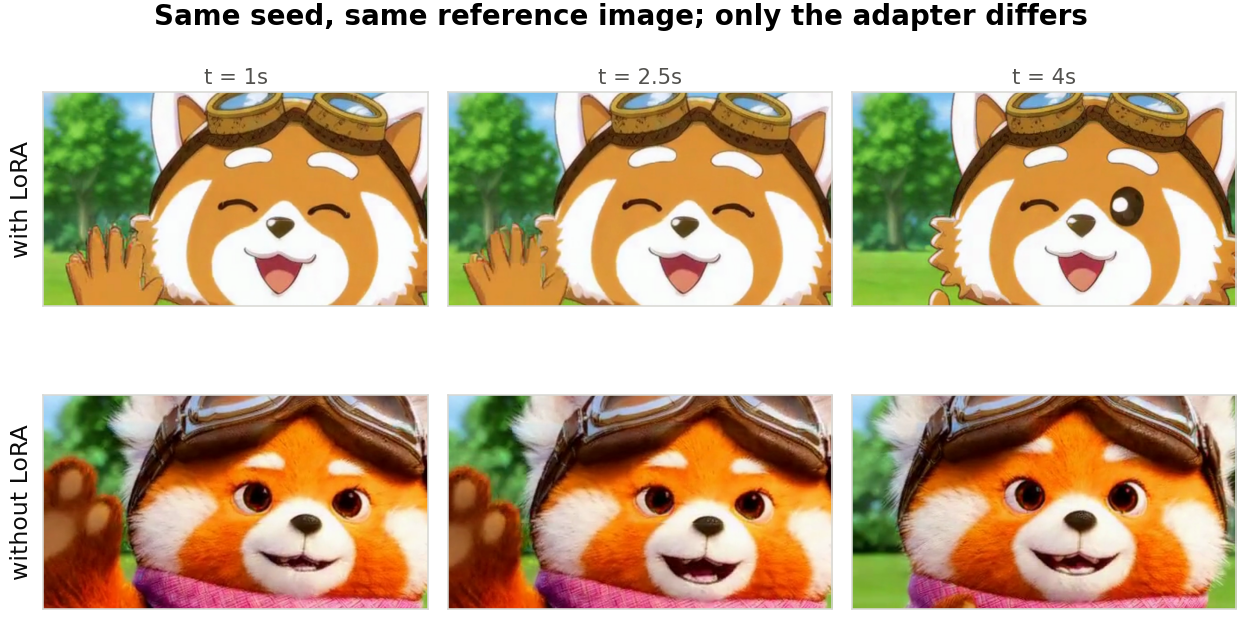
\includegraphics[width=\linewidth]{figures/fig_ablation_frames.png}
\caption{Same seed, same reference image, adapter toggled. The top row renders as flat illustration; the bottom row renders individual strands of fur.}
\label{fig:abframes}
\end{figure*}

The roles separate cleanly: \emph{the reference image carries what is drawn; the LoRA carries how it is drawn.} ``A reference image makes the LoRA unnecessary'' is therefore false. The return on a character LoRA is not the ability to render the character---it is the ability to render it \textbf{in one's own style}.

\subsection{Strength and training length}

Twenty-four clips spanning strength 0.0--1.2 and checkpoints 300--800 were generated under fixed conditions and evaluated qualitatively (Figures~\ref{fig:strength} and~\ref{fig:checkpoint}).

\begin{figure}[t]
\centering
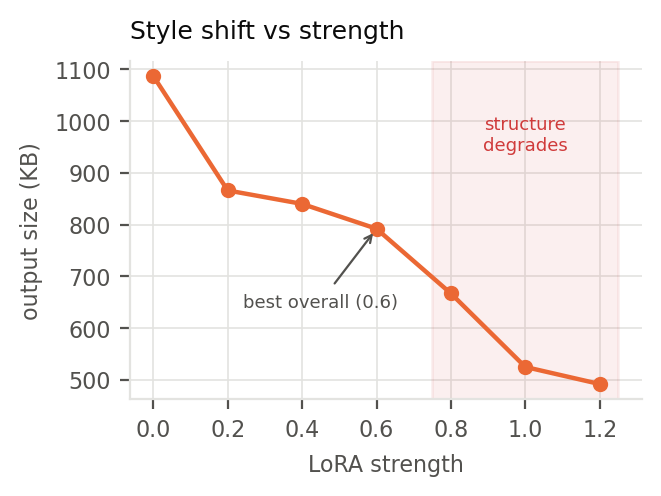
\includegraphics[width=\linewidth]{figures/fig_strength.png}
\caption{Style shift against adapter strength. Output size serves as a proxy for how far the style has moved.}
\label{fig:strength}
\end{figure}

\begin{figure}[t]
\centering
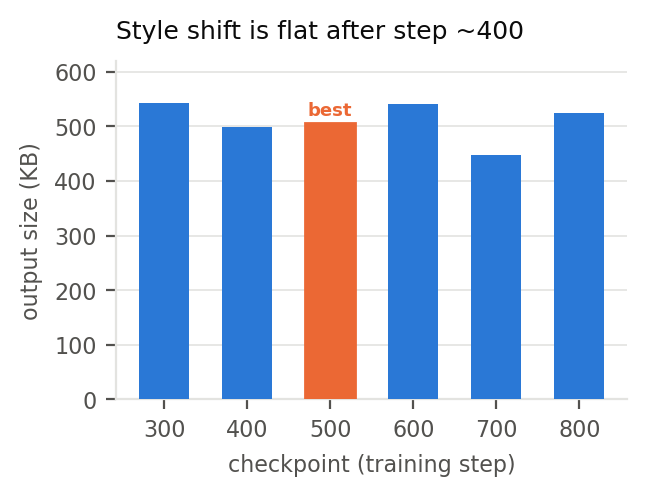
\includegraphics[width=\linewidth]{figures/fig_checkpoint.png}
\caption{Effect of training length. Style shift plateaus after roughly step 400.}
\label{fig:checkpoint}
\end{figure}

\textbf{Style fidelity and structural accuracy move in opposite directions.} Raising strength moves the style toward the target while degrading complex regions---hands above all. Training length plateaus near step 500; later steps add nothing, and step 700 showed mild degradation.

\subsection{Cross-validation and the recommended setting}

The two sweeps above were run at fixed values of the other axis---strength at step 800, checkpoints at strength 1.0---leaving the combination of the two best values untested. Generating strengths 0.6, 0.8 and 1.2 at checkpoint 500 closed that gap.

\textbf{Checkpoint 500 at strength 0.8 was best overall.} At 0.6 the style has not moved far enough. At 1.2 the style is closest to target, but \emph{a heavy dark contour appears around the whole character}---a faithful reproduction of the die-cut border in the sticker artwork used for training. Natural in a sticker, it reads as an artifact in video.

\begin{figure*}[t]
\centering
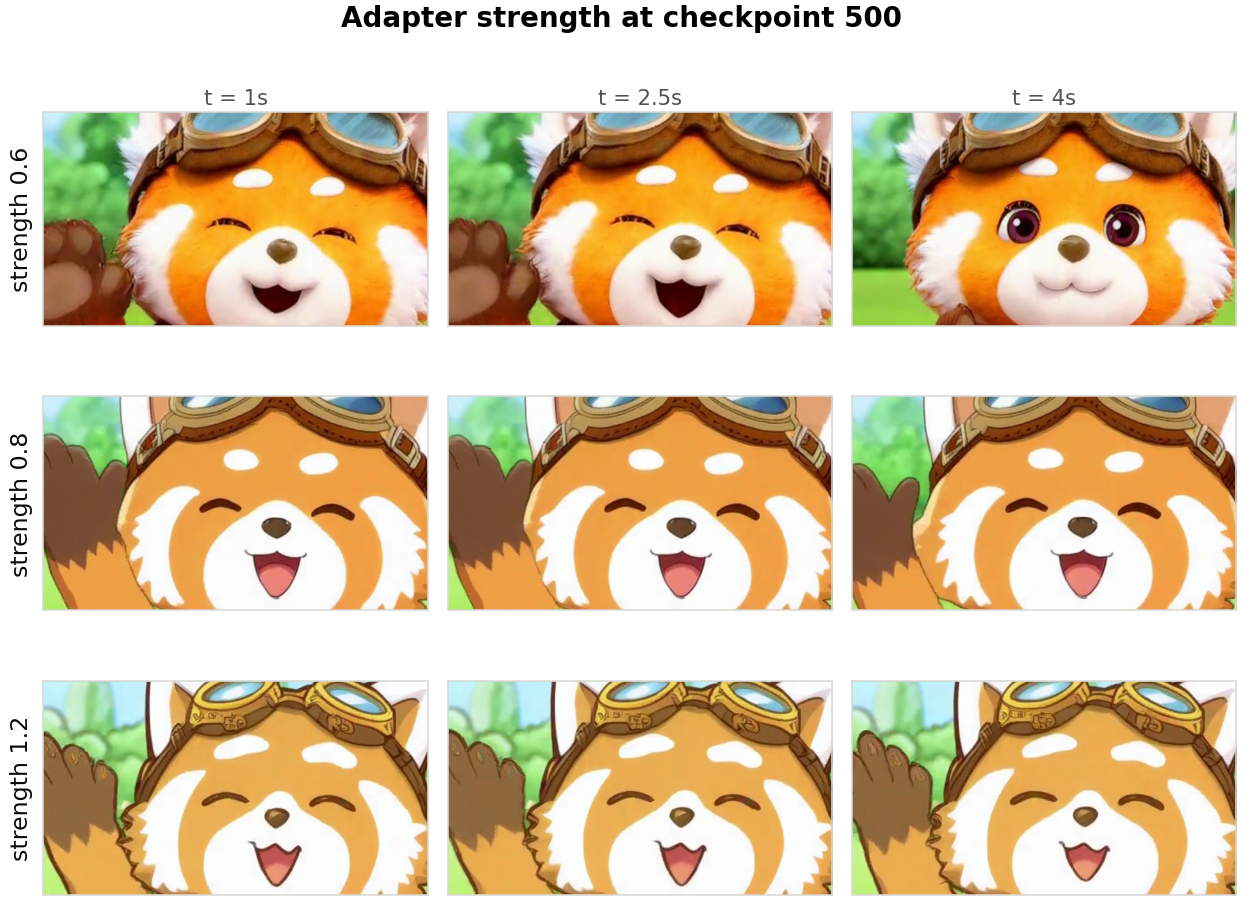
\includegraphics[width=\linewidth]{figures/fig_strength_frames.png}
\caption{Adapter strength at checkpoint 500. At 1.2 a heavy dark contour wraps the whole character.}
\label{fig:stframes}
\end{figure*}

The recommendation is therefore \textbf{500 steps at strength 0.8}, and the initially chosen 800 steps at strength 1.0 was \emph{excessive in both training and inference}. Training drops from about two hours to about 1.25, and cost from \$1.89 to roughly \$1.2.

\subsection{What the dataset smuggles in}

Cross-validation surfaced three ways the adapter carries properties of the training data that were never asked for.

First, the \textbf{contour} described above.

Second, \textbf{fine detail needs strength}. Captions read \texttt{pink patterned scarf}, yet at strengths 0.6 and 0.8 the scarf is nearly plain; the pattern appears only at 1.2.

Third, \textbf{the adapter reshapes backgrounds too}. A depth-blurred background at 0.6 becomes graphic linework at 1.2. Captions described whole images, so the learned style spans the frame---too broad a reach if the goal is to swap only the character.

Each of these shows \emph{caption design and dataset provenance surfacing directly as properties of the output}.

\subsection{The trigger token}

Removing the trigger while keeping the appearance description preserved the elements but lost the style. Supplying the trigger alone, with no appearance description, failed to produce a usable result. \textbf{The adapter does not fully internalize the appearance; the caption text is doing real work.} With only 12 training images, all captioned with the same appearance clause, this is the expected outcome.

\subsection{On output size as a proxy}

Output file size decreased monotonically with strength, from 1{,}087\,KB at 0.0 to 492\,KB at 1.2. The training art is flat-shaded, so as the style converges the tonal range narrows and the codec compresses better.

Size is nonetheless \textbf{not a quality metric}. The smallest outputs---strength 1.2 and checkpoint 700---were exactly the ones carrying structural breakage or artifacts. Size measures style displacement and nothing else.

\section{Limitations}

\begin{enumerate}[leftmargin=1.6em,topsep=2pt,itemsep=2pt]
  \item \textbf{Peak system RAM during training was never measured.} The monitor recorded GPU statistics only. The requirement can therefore be stated as a range---above 50\,GB, at or below 188\,GB---and no more precisely. Instrumentation has since been added.
  \item \textbf{Cost is approximate.} The account balance before the A40 attempts was not recorded, so the total is stated as about five dollars; the span measurable through the API was \$3.44.
  \item \textbf{Qualitative evaluation came from a single rater} without blinding.
  \item \textbf{The dataset holds 12 images.} Conclusions about the trigger token and about generalization may be specific to that scale.
  \item \textbf{Generalization to unseen scenes was limited.} In settings absent from training---a neon street at night, riding a bicycle---the adapter degraded detail relative to the un-adapted baseline.
\end{enumerate}

\section{Conclusion}

For LoRA training of a 33B omni-modal video model, the binding constraint was \textbf{system RAM}, not VRAM (Q1). Peak VRAM measured 3{,}959\,MiB---2.8\% of the installed card---while 50\,GB of system RAM failed during loading and 188\,GB completed.

The claim carried by the two earlier studies~\cite{suzuki2026sd15lora,suzuki2026krea2lora}---that a single consumer GPU suffices---\textbf{does not hold at this scale}. But it fails for a reason other than the expected one: not too little VRAM, too little system RAM. What one should rent is therefore not a GPU with large VRAM but \textbf{a machine with large system RAM}, and because advertised RAM tracks neither price nor VRAM, that has to be checked deliberately.

The trained adapter transfers across quantization formats and infers within 9.3\,GB of VRAM (Q2), so \textbf{training can be rented while operation stays on local consumer hardware}.

Under reference-image conditioning the adapter contributes style rather than structural stability (Q3). Strength trades style fidelity against structural accuracy, and cross-validation puts the optimum at \textbf{500 steps, strength 0.8}. The initial choice was excessive.

Total compute cost was about five US dollars.

\section*{Reproducibility}

Scripts, dataset, measurement logs and the source of this paper are published at:

\begin{itemize}[leftmargin=1.4em,topsep=2pt,itemsep=0pt]
\item \url{https://github.com/masafykun/minimax-h3-masafy-lora}
\item \url{https://huggingface.co/masafy/minimax-h3-masafy-lora}
\end{itemize}

\begin{thebibliography}{9}
\bibitem{suzuki2026sd15lora} M.~Suzuki. Character LoRA Fine-tuning for Image Generation: An Experimental Study under Few-shot Conditions on a Consumer GPU. Technical report, 2026.
\bibitem{suzuki2026krea2lora} M.~Suzuki. Character LoRA Fine-tuning of a 12B Image Generation Model: FP8 Quantization and Block Swapping on a Single Consumer GPU, with Transfer to a Distilled Model. Technical report, 2026. DOI: 10.5281/zenodo.20838898.
\bibitem{hu2022lora} E.~J.~Hu, Y.~Shen, P.~Wallis, Z.~Allen-Zhu, Y.~Li, S.~Wang, L.~Wang, and W.~Chen. LoRA: Low-Rank Adaptation of Large Language Models. \textit{International Conference on Learning Representations (ICLR)}, 2022.
\bibitem{peebles2023dit} W.~Peebles and S.~Xie. Scalable Diffusion Models with Transformers. \textit{IEEE/CVF International Conference on Computer Vision (ICCV)}, 2023.
\bibitem{lipman2023flowmatching} Y.~Lipman, R.~T.~Q. Chen, H.~Ben-Hamu, M.~Nickel, and M.~Le. Flow Matching for Generative Modeling. \textit{International Conference on Learning Representations (ICLR)}, 2023.
\bibitem{ruiz2023dreambooth} N.~Ruiz, Y.~Li, V.~Jampani, Y.~Pritch, M.~Rubinstein, and K.~Aberman. DreamBooth: Fine Tuning Text-to-Image Diffusion Models for Subject-Driven Generation. \textit{IEEE/CVF Conference on Computer Vision and Pattern Recognition (CVPR)}, 2023.
\bibitem{qwenimage2025} Qwen Team. Qwen-Image Technical Report. 2025.
\bibitem{aitoolkit2026} ostris. AI Toolkit. \url{https://github.com/ostris/ai-toolkit}, 2026.
\bibitem{comfyui2026} comfyanonymous. ComfyUI. \url{https://github.com/comfyanonymous/ComfyUI}, 2026.
\end{thebibliography}

\end{document}
